%%%%%%%%%%%%%%%%%%%%%%%%%%%%%%%%%%%%%%%%%%%%%%%%%%%
% A small project to practice LaTeX and Git
% N. Westerlund
% April 17, 2026
%%%%%%%%%%%%%%%%%%%%%%%%%%%%%%%%%%%%%%%%%%%%%%%%%%%

% another comment

%simulating a change from someone else

\documentclass[a4paper,11pt]{article}

\usepackage[T1]{fontenc}
\usepackage[default]{sourcesans}
\usepackage{sourcecodepro}

\usepackage[
  left=1.2cm,
  right=1.2cm,
  top=1.2cm,
  bottom=1.2cm
]{geometry}

\usepackage{graphicx}

\setlength{\parindent}{0pt}
\setlength{\parskip}{0pt}

\title{Git Workflow Cheat Sheet for LaTeX Collaborators}
\author{Nils Westerlund}
\date{} % Don't print date and prevent \maketitle to adding date

\begin{document}
\pagestyle{empty}

\maketitle
\thispagestyle{empty}

\section*{MENTAL MODEL}

% A comment
\begin{itemize}
  \renewcommand{\labelitemi}{$\rightarrow$}
    \item A commit = a snapshot of tracked files.
    \item A branch = a label pointing to a line of commits.
    \item main = the shared stable branch.
    \item origin = the remote repository nickname.
    \item origin/main = your local record of the remote main branch.
    \item fetch updates your record of the remote; it does not change your files.
\end{itemize}   

\section*{GIT WORKFLOW OVERVIEW}
The Git workflow helps structure collaboration by separating stable code in \texttt{main} from ongoing work in feature branches. Changes are developed, committed in small steps, and regularly synchronized with the latest version of \texttt{main} to avoid conflicts. This process ensures a clean history and reliable integration of contributions. Figure~\ref{fig:git-workflow} provides a visual overview of this workflow and the associated commands.

\begin{figure}[!htbp]
  \centering
  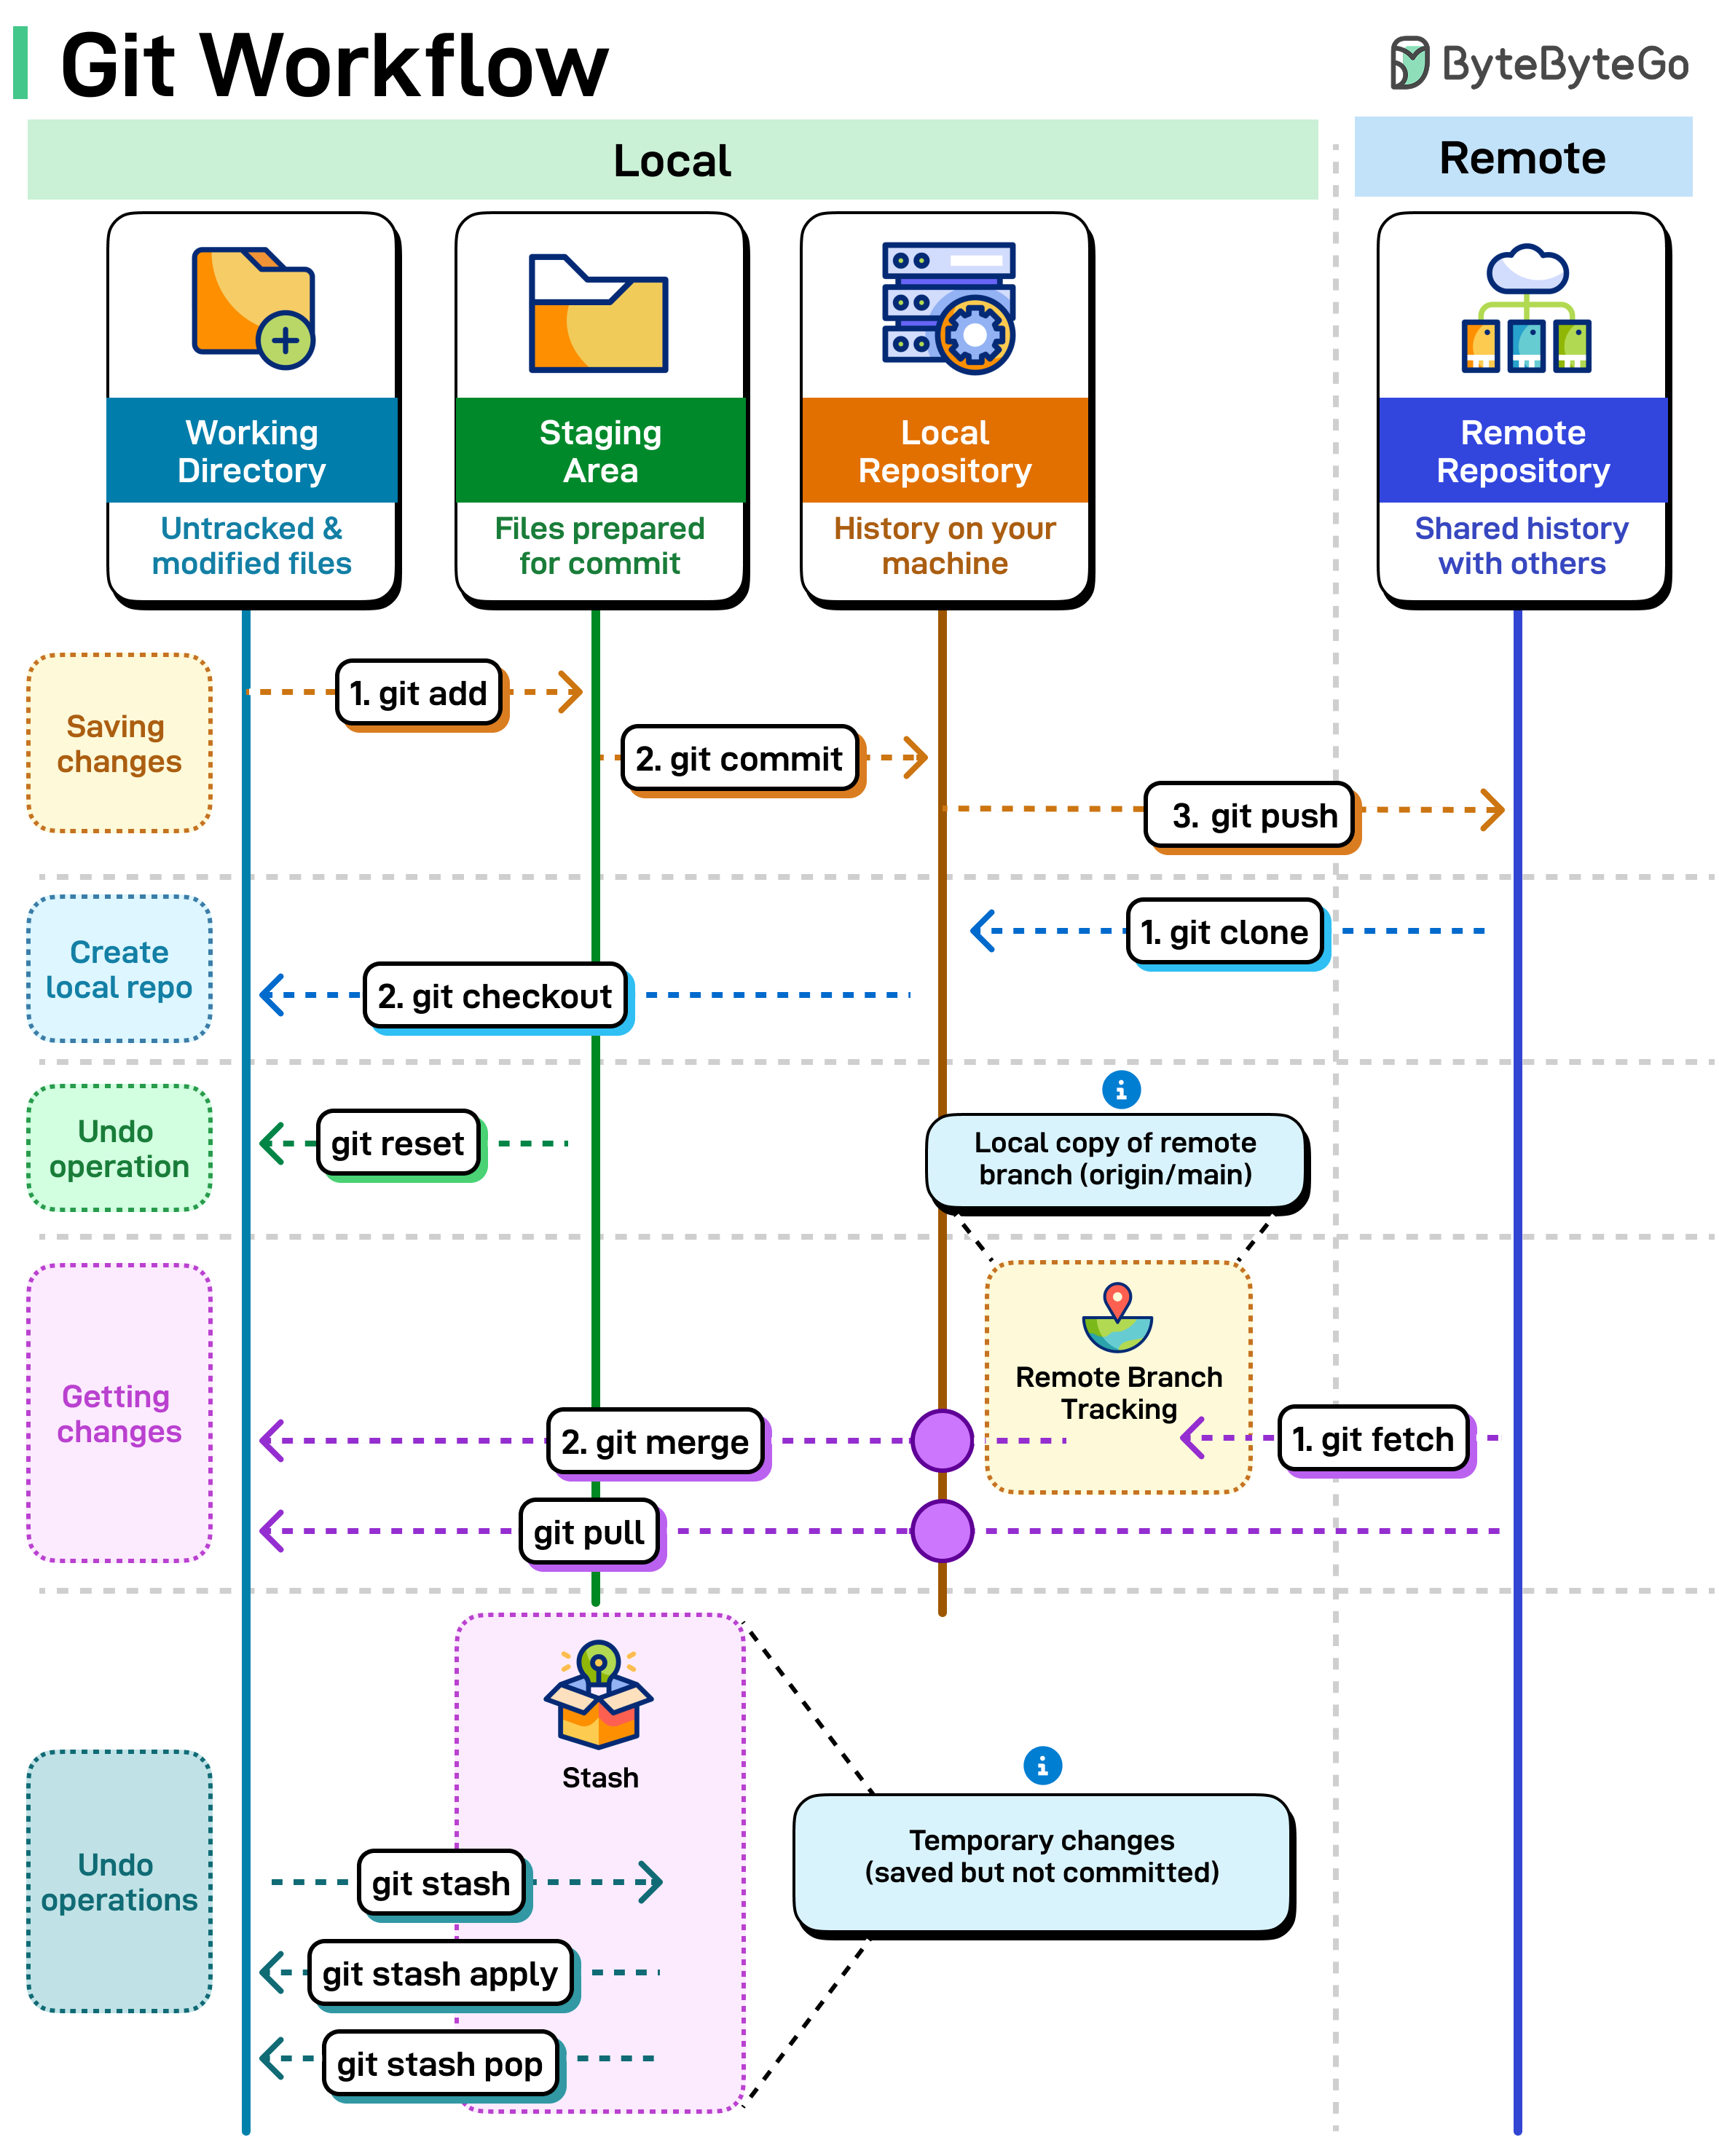
\includegraphics[width=0.5\textwidth]{images/git_workflow_overview.png}
  \caption{An overview of the git workflow with associated commands.}
  \label{fig:git-workflow}
\end{figure}
% simulating an update to figure caption

\section*{CORE SAFE WORKFLOW}

\begin{itemize}
  \renewcommand{\labelitemi}{$\rightarrow$}

  \item Update local main
    \begin{itemize}
      \renewcommand{\labelitemii}{$\triangleright$}
      \item \texttt{git switch main}
      \item \texttt{git pull --ff-only}
    \end{itemize}

  \item Create a branch for one task
    \begin{itemize}
      \renewcommand{\labelitemii}{$\triangleright$}
      \item \texttt{git switch -c fix-bibliography}
    \end{itemize}

  \item Work normally
    \begin{itemize}
      \renewcommand{\labelitemii}{$\triangleright$}
      \item edit \texttt{.tex} / \texttt{.bib} / figures
      \item compile and check output
      \item inspect changes:
        \begin{itemize}
          \item \texttt{git status}
          \item \texttt{git diff}
        \end{itemize}
    \end{itemize}

  \item Commit in small logical chunks
    \begin{itemize}
      \renewcommand{\labelitemii}{$\triangleright$}
      \item \texttt{git add sections/intro.tex references.bib}
      \item \texttt{git commit -m "Fix bibliography keys and citations"}
    \end{itemize}

  \item Sync with teammates before pushing / opening PR
    \begin{itemize}
      \renewcommand{\labelitemii}{$\triangleright$}
      \item \texttt{git fetch origin}
      \item \texttt{git rebase origin/main}
    \end{itemize}

  \item Push your branch
    \begin{itemize}
      \renewcommand{\labelitemii}{$\triangleright$}
      \item \texttt{git push -u origin fix-bibliography}
    \end{itemize}

  \item Open a pull request / merge request

  \item After merge
    \begin{itemize}
      \renewcommand{\labelitemii}{$\triangleright$}
      \item \texttt{git switch main}
      \item \texttt{git pull --ff-only}
      \item \texttt{git branch -d fix-bibliography}
    \end{itemize}

\end{itemize}




\section*{DAILY COMMANDS}

\begin{tabular}{@{}l l@{}}
Check status            & \texttt{git status} \\
See unstaged changes    & \texttt{git diff} \\
Stage files             & \texttt{git add <files>} \\
Commit snapshot         & \texttt{git commit -m "Meaningful message"} \\
See branches            & \texttt{git branch} \\
                        & \texttt{git branch -a} \\
Push current branch     & \texttt{git push} \\
\end{tabular}

\section*{FETCH / PULL / MERGE / REBASE}

\begin{tabular}{@{}l l@{}}
\texttt{git fetch origin} & downloads new commits and updates \texttt{origin/main} \\
                          & does NOT modify your working files \\[0.5em]

\texttt{git pull --ff-only} & updates current branch only if it can move straight forward \\
                            & safest way to update \texttt{main} \\[0.5em]

\texttt{git merge origin/main} & combines histories with a merge commit \\
                               & good when you want to avoid rewriting your branch history \\[0.5em]

\texttt{git rebase origin/main} & replays your branch commits on top of latest \texttt{main} \\
                                & keeps history cleaner \\
                                & best for your own local feature branches \\
\end{tabular}

\section*{GOOD TEAM RULES}

\begin{itemize}
  \renewcommand{\labelitemi}{$\rightarrow$}
  \item Keep main buildable.
  \item Use one branch per task.
  \item Prefer small, focused commits.
  \item Rebase your own feature branch if needed.
  \item Do not rebase shared branches people already use.
  \item Never force-push main.
  \item Open a PR instead of pushing directly to main when collaborating.
\end{itemize}

\section*{LATEX-SPECIFIC ADVICE}

\begin{itemize}
  \renewcommand{\labelitemi}{$\rightarrow$}

  \item Split large documents into files:
    \begin{itemize}
      \renewcommand{\labelitemii}{$\triangleright$}
      \item \texttt{sections/introduction.tex}
      \item \texttt{sections/methods.tex}
      \item \texttt{sections/results.tex}
    \end{itemize}

  \item Keep generated build files out of Git with \texttt{.gitignore}. \\
        Common ignores:
    \begin{itemize}
      \renewcommand{\labelitemii}{$\triangleright$}
      \item \texttt{*.aux}
      \item \texttt{*.bbl}
      \item \texttt{*.blg}
      \item \texttt{*.fdb\_latexmk}
      \item \texttt{*.fls}
      \item \texttt{*.log}
      \item \texttt{*.out}
      \item \texttt{*.synctex.gz}
      \item \texttt{*.toc}
      \item \texttt{*.pdf}
    \end{itemize}

  \item Avoid mass reformatting while others edit content.
  \item Commit working builds when possible.

\end{itemize}

\section*{COMMON FLOWS}

\begin{itemize}
  \renewcommand{\labelitemi}{$\rightarrow$}

  \item Start new work
    \begin{itemize}
      \renewcommand{\labelitemii}{$\triangleright$}
      \item \texttt{git switch main}
      \item \texttt{git pull --ff-only}
      \item \texttt{git switch -c branch-name}
    \end{itemize}

  \item Save progress
    \begin{itemize}
      \renewcommand{\labelitemii}{$\triangleright$}
      \item \texttt{git add <files>}
      \item \texttt{git commit -m "Describe the change"}
    \end{itemize}

  \item Update your feature branch with latest main
    \begin{itemize}
      \renewcommand{\labelitemii}{$\triangleright$}
      \item \texttt{git fetch origin}
      \item \texttt{git rebase origin/main}
    \end{itemize}

  \item Publish your branch
    \begin{itemize}
      \renewcommand{\labelitemii}{$\triangleright$}
      \item \texttt{git push -u origin branch-name}
    \end{itemize}

\end{itemize}

\section*{USEFUL RECOVERY COMMANDS}

\begin{itemize}
  \renewcommand{\labelitemi}{$\rightarrow$}

  \item Unstage a file
    \begin{itemize}
      \renewcommand{\labelitemii}{$\triangleright$}
      \item \texttt{git restore --staged <file>}
    \end{itemize}

  \item Discard unstaged changes in a file
    \begin{itemize}
      \renewcommand{\labelitemii}{$\triangleright$}
      \item \texttt{git restore <file>}
    \end{itemize}

  \item Show history clearly
    \begin{itemize}
      \renewcommand{\labelitemii}{$\triangleright$}
      \item \texttt{git log --oneline --graph --decorate --all}
    \end{itemize}

\end{itemize}

\section*{FINAL TAKEAWAY}

\begin{itemize}
  \renewcommand{\labelitemi}{$\rightarrow$}

  \item For each task:
    \begin{itemize}
      \renewcommand{\labelitemii}{$\triangleright$}
      \texttt{main $\rightarrow$ pull $\rightarrow$ new branch $\rightarrow$ work $\rightarrow$ commit $\rightarrow$ fetch $\rightarrow$ rebase $\rightarrow$ push $\rightarrow$ PR}
    \end{itemize}

\end{itemize}


\end{document}
